
\documentclass[runningheads,a4paper]{llncs}

\usepackage[utf8]{inputenc}            % kodowanie
\usepackage[OT4]{fontenc}              % font PL
\usepackage[polish]{babel}
% \usepackage{amssymb}
% \usepackage{minted}
\usepackage{listings}
\usepackage{color}
\setcounter{tocdepth}{3}
\usepackage{graphicx}
\usepackage{epstopdf}
\usepackage{caption}
\captionsetup{compatibility=false}
\captionsetup{justification=centering}
\usepackage{subcaption}
\setcounter{secnumdepth}{3}

\definecolor{mygreen}{rgb}{0,0.6,0}
\definecolor{mygray}{rgb}{0.5,0.5,0.5}
\definecolor{mymauve}{rgb}{0.58,0,0.82}
\definecolor{mygrey}{rgb}{0.97,0.97,0.97}

\lstset{
  backgroundcolor=\color{mygrey},   % choose the background color; you must add \usepackage{color} or \usepackage{xcolor}
  basicstyle=\footnotesize\ttfamily,        % the size of the fonts that are used for the code
  breakatwhitespace=false,         % sets if automatic breaks should only happen at whitespace
  breaklines=true,                 % sets automatic line breaking
  captionpos=b,                    % sets the caption-position to bottom
  aboveskip=0pt,
  abovecaptionskip=0pt,
  commentstyle=\color{mygreen},    % comment style
  deletekeywords={...},            % if you want to delete keywords from the given language
  escapeinside={\%*}{*)},          % if you want to add LaTeX within your code
  extendedchars=true,              % lets you use non-ASCII characters; for 8-bits encodings only, does not work with UTF-8
%   frame=single,                    % adds a frame around the code
  framexleftmargin=3pt,
  framexbottommargin=3pt,
  framextopmargin=0pt,
  framexrightmargin=3pt,
  framerule=0.1pt,
   language=Octave,
  keepspaces=true,                 % keeps spaces in text, useful for keeping indentation of code (possibly needs columns=flexible)
  keywordstyle=\color{blue},       % keyword style
%   morekeywords={*,...},            % if you want to add more keywords to the set
  numbers=left,                    % where to put the line-numbers; possible values are (none, left, right)
  numbersep=8pt,                   % how far the line-numbers are from the code
  numberstyle=\footnotesize\color{mygray}, % the style that is used for the line-numbers
  rulecolor=\color{black},         % if not set, the frame-color may be changed on line-breaks within not-black text (e.g. comments (green here))
  showspaces=false,                % show spaces everywhere adding particular underscores; it overrides 'showstringspaces'
  showstringspaces=false,          % underline spaces within strings only
  showtabs=false,                  % show tabs within strings adding particular underscores
  stepnumber=1,                    % the step between two line-numbers. If it's 1, each line will be
  stringstyle=\color{mymauve},     % string literal style
  tabsize=4,                       % sets default tabsize to 2 spaces
  title=\lstname                   % show the filename of files included with \lstinputlisting; also try caption instead of title
}


\usepackage{url}
\urldef{\mailsa}\path|{alfred.hofmann, ursula.barth, ingrid.haas, frank.holzwarth,|
\urldef{\mailsb}\path|anna.kramer, leonie.kunz, christine.reiss, nicole.sator,|
\urldef{\mailsc}\path|erika.siebert-cole, peter.strasser, lncs}@springer.com|
\newcommand{\keywords}[1]{\par\addvspace\baselineskip
\noindent\keywordname\enspace\ignorespaces#1}

\renewcommand{\keywordname}{\textbf{Słowa kluczowe:}}

\setlength{\fboxsep}{0pt}
\setlength{\fboxrule}{1pt}

\begin{document}

\mainmatter
\title{Wykrywanie ataków w sieciach komputerowych z wykorzystaniem systemów Honeypot}
\author{Maciej Jagiełło}

\titlerunning{ }
\authorrunning{ }
\institute{}
\maketitle

\begin{abstract}
A tu będzie streszczenie!!!!!!!!!!!!!!!!!!!!!!!!!!!!!!1
\keywords{honeypot, glastopf, kippo, dionaea, vagrant, puppet, virtualbox}
\end{abstract}


\section{Wprowadzenie}

Wykrywanie ataków w sieciach komputerowych to ważny element działań na rzecz zwiększania bezpieczeństwa systemów. Cyberprzestępczość rozwija się szybkim tempem. Z każdym dniem opracowywane są nowe sposoby ataków, wykorzystywane są nowe podatności w aplikacjach, protokołach i systemach operacyjnych. Aby temu przeciwdziałać, konieczne jest opracowanie odpowiednich narzędzi. ....

Celem systemu jest stworzenie narzędzia do zbierania adresów IP hakerów, botów i zainfekowanych maszyn w spójną bazę danych, którą będzie można później wykorzystać np. do rozszerzania reguł zapór ogniowych. System ma być też źródłem nowych wirusów do analizowania przez antywirusy. Wybrane rozwiązanie problemu to sieć Honeypotów.

Honeypot to jedynie idea zbierania informacji. Jest to kombinacja ustawień sprzętowych i programowych, które tworzą system pułapkę. Ustawienia sprzętowe, czyli komputer, wyodrębniony obszar sieci lokalnej, który odpowiednio symuluje prawdziwą sieć, ale jest od niej odizolowany i zabezpieczony.

Taki system, uruchomiony na maszynie serwerowej, udostępnia w Internecie jakiś zasób atrakcyjny dla atakującego. Może to być rekord w bazie danych, aplikacja lub cały system operacyjny. Używając odpowiednich mechanizmów do monitorowania zachowania, zbiera dane o sposobach wykonywania ataków.

Jego główną zaletą jest to, że korzystają z niego niemal wyłącznie użytkownicy, którzy chcą włamać się do sieci.

\section{Sieć honeypotów}

Na rysunku \ref{fig:architektura_fig} przedstawiony jest schemat architektury aplikacji. Każdy honeypot uruchomiony jest w maszynie wirtualnej. Maszyna ta posiada dostęp do Internetu i wystawia do niego, odpowiednie dla zainstalowanych honeypotów, zasoby. Moduł pobierania i analizy logów zbiera pozostawione przez honeypoty informacje o atakujących. Są to ślady wykonywanych akcji i pliki binarne ładowane na maszyny przez atakujących.

\begin{figure}
        \centering
        \fbox{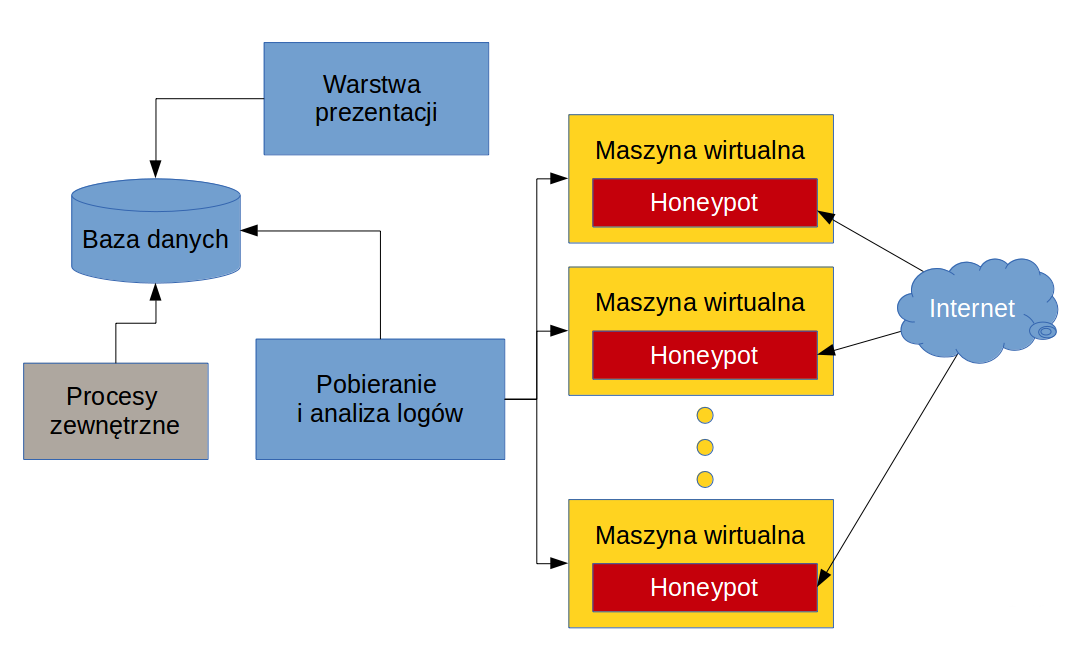
\includegraphics[width=1.0\textwidth]{pics/architektura}}
        \caption{Architektura aplikacji.}
        \label{fig:architektura_fig}
\end{figure}

Istnieje bardzo dużo realizacji honeypotów. Na stronie \cite{honeynet_project}, która zajmuje się rozwojem narzędzi do zwiększenia bezpieczeństwa w internecie, jest wymienione około 30 projektów, a to z pewnością nie wszystkie dostępne.

Warto wspomnieć o pracującym na wydziale Elektroniki i Technik Informacyjnych, doktorze Krzysztofie Cabaju, który na przedmiotach BSS, SKM2 i TKOM prowadzi studentów podczas implementacji autorskich honeypotów.

W opisywanym systemie zostały wybrane trzy realizacje honeypotów ze względu na wystarczającą różnorodność w oferowanych przez nie usługach.

\section{Honeypoty}

\subsection{Glastopf}
Pierwszy z prezentowanych honeypotów, Glastopf, jest zwykłą stroną www, którą można znaleźć w wyszukiwarkach internetowych. Treść strony zawiera frazy w języku angielskim, które są generowane z dostarczonej przez twórców bazy danych. Glastopf potrafi w prosty sposób analizować zapytania HTTP, w szczególności te zapytania GET, które w adresie URL zawierają inne adresy URL do zewnętrznych plików. Takie argumenty parsuje i próbuje ściągać na dysk do późniejszej analizy.

\subsection{Kippo}

Kolejnym wektorem ataków, na jaki są podatne komputery w sieciach komputerowych jest protokół ssh. Kippo symuluje sesję SSH udostępniając prostego shella. Najczęściej używane polecenia mają napisane własne implementacje, które oszukują użytkownika tego środowiska. Polecenia rzadziej używane zwracają błąd, w taki sposób, aby nie zdradzić fałszywości systemy. Kippo udostępnia dla nich fałszywy system plików tylko do odczytu, który wygląda jak po świeżej instalacji Debiana.

Ta aplikacja loguje informacje o adresach IP, próbach pobrania plików z Internetu, zapisuje te pliki w kwarantannie, oraz loguje całą sesję użytkownika od próby zalogowania na serwer, aż do aktywności po wylogowaniu. Robi to przechwytując polecenia „logout“, „exit“ lub znak wysyłany kombinacją klawiszy Ctrl + D. Następnie wyświetla znak zachęty wyglądający jak na lokalnym komputerze.

\subsection{Dionaea}

Ostatnim z użytych w systemie honeypotów jest Dionaea. Protokoły, którymi się posługuje do serwowania pułapki to głównie Samba, HTTP, FTP, MySQL, RTP. Samba jest bardzo popularnym protokołem do wymiany plików w Windowsie. Wiele osób bez zaawansowanej wiedzy o tym systemie korzysta z niego i nieumyślnie otwiera sobie drogę do włamania. Dlatego atakujący często szukają drogi właśnie tym kanałem.

\section{Środowisko uruchomieniowe}

Istotnym, choć niekoniecznym krokiem w stronę bezpieczeństwa systemu jest uruchamianie serwerów honeypotowych w maszynie wirtualnej. Pozwala to osiągnąć wysoki poziom separacji środowiska podatnego na ataki, od rzeczywistej maszyny, nad którą nie można stracić dostępu. Dodatkowo to rozwiązanie jest bardzo przydatne gdy jest potrzeba, by system był łatwy w replikacji na inne maszyny. Aplikacja uruchamiająca maszynę wirtualną jest odpowiedzialna za dostarczenie takiego samego środowiska. W opisywanym systemie tą aplikacją jest VirtualBox rozwijany przez firmę Oracle.

Dodatkową warstwą nad VirtualBoxem jest Vagrant. Jest to świetne narzędzie do automatyzacji instalacji maszyny wirtualnej z użyciem skryptów konfiguracyjnych. Jego użycie polega na przygotowaniu skryptu instalacyjnego na naszej maszynie. W tym systemie do instalacji honeypotów został użyty Puppet. Puppet to narzędzie do deklaratywnego zarządzania stanem maszyny.

Alternatywą do wirtualnej maszyny jest wirtualny kontener, który nie tworzy wirtualnego systemu od początku do końca, a tylko izoluje aplikację od systemu. Najpopularniejszym rozwiązaniem jest Docker. Docker potrzebuje mniej zasobów systemowych, ale nie gwarantuje 100\% bezpieczeństwa.

\subsection{Narzędzia}

Wartym do wejścia w szczegóły tematem jest wspólne działanie Vagranta, VirtualBoxa i Puppeta. Schemat jest przedstawiony na rysunku \ref{fig:vagrant_fig}. Numery obok strzałek oznaczają kolejne kroki instalacji honeypota na maszynie wirtualnej.

Zanim można rozpocząć procedurę, należy pobrać dystrybucję systemu poleceniem \texttt{vagrant init}:
\begin{lstlisting}
$ vagrant init hashicorp/precise32
\end{lstlisting}

Następnie polecenie \texttt{vagrant up} uruchamia procedurę. Najpierw Vagrant, korzystając z VirtualBoxa tworzy wirtualne środowisko. Potem uruchamia skrypty Puppetowe. One instalują się na maszynie tworząc gotowe środowisko.

Dostęp do stworzonej maszyny można uzyskać poprzez polecenie \texttt{vagrant ssh}.

\begin{figure}
        \centering
        \fbox{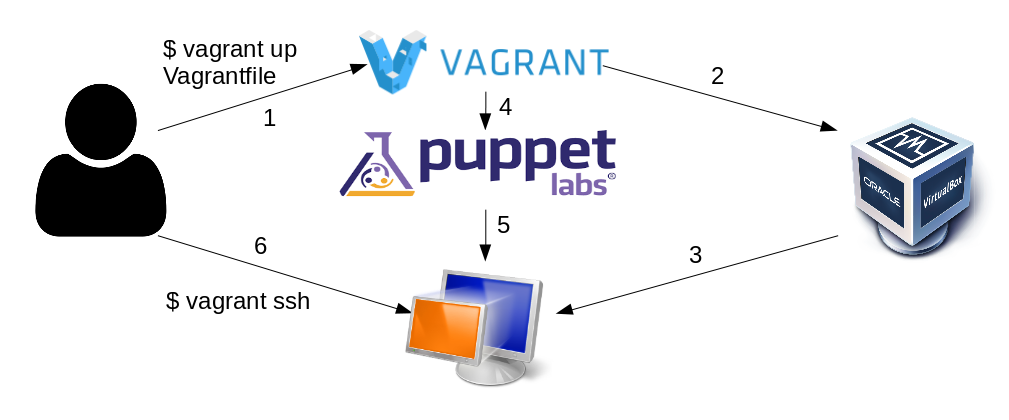
\includegraphics[width=1.0\textwidth]{pics/vagrant}}
        \caption{Vagrant, Puppet, VirtualBox.}
        \label{fig:vagrant_fig}
\end{figure}

Cały proces trwa około 5 minut, został wykonany z użyciem 3 poleceń w terminalu, a wynikiem jest maszyna wirtualna z ubuntu server w 32 bitowej wersji z zainstalowanym honeypotem.

\subsection*{Puppet}

Przykładowy i skrócony na potrzeby artykułu plik puppetowy w listingu \ref{glastopf_file}.
\\
\lstinputlisting[caption={glastopf.pp},label={glastopf_file}]{code/glastopf.pp}

Kolejność, moduły, bashe (również warunki na OS), serwisy, paczki z pipa apt-geta niezależnie od systemu i bez promptów o hasło czy potwierdzenie kontynuacji

Wystarczy puppet apply

Możliwa architektura master-slave, ale nie używana w tym projekcie

\section{}
Aplikacja
Silnik zbierania danych napisany w Javie
Metadane o każdym honeypocie:
Lista lokalizacji plików do ściągnięcia
Reguły rozpoznawania plików tekstowych
Testy integracyjne z użyciem Vagranta, Virtualboxa i Puppeta
\section{}
Pierwszym problemem przy pobieraniu logów jest to, że ze względów bezpieczeństwa honeypot nie powinien mieć dostępu do żadnej części tworzonego systemu, ponieważ w przypadku włamania się na serwer, haker może zniszczyć nie tylko maszynę z honeypotem.

Najprostszym sposobem wyciągania logów jest użycie protokołu ssh. Nie wymaga instalowania dodatkowych aplikacji, wspiera przesyłanie plików, jest protokołem względnie bezpiecznym w porównaniu do innych autorskich rozwiązań.

Aby poradzić sobie z rosnącym w nieskończoność plikiem logów, trzeba go albo czyścić albo archiwizować.

\section{}
Dwa przykłady prezentacji na żywo ataków z sieci honeypotów.

Typy ataków, ip (lokacja), geoIP, live

To tylko warstwa prezentacji
\section{Podsumowanie}
Użyłem honeypotów ..., spełniły swoje zadanie. Pierwsze dane od botów skanujących internet pojawiły się już po paru dniach. Teraz jest to jakieś 500 ataków na godzinę.

Wdrażanie ich to proste uruchomienie skryptu.

Najczęściej spotyka się boty o nagłówkach HTTP, że to tylko zbieranie danych na potrzeby badań - „edukacyjne“

\section{}
\begin{thebibliography}{1}

% \bibitem{url} Xa,
% \url{http://xa}

\bibitem{} Ataki sieciowe,
\url{http://jbeczala.republika.pl/files/ataki_sieciowe.pdf}
\bibitem{honeynet_project} l, \url{https://www.honeynet.org/project}
\bibitem{} l,
\url{http://glastopf.org/}
\bibitem{} k,
\url{https://github.com/desaster/kippo}
\bibitem{} j,
\url{https://www.honeynet.org/project}
\bibitem{} h,
\url{http://map.ipviking.com/}
\bibitem{} g,
\url{http://digitalattackmap.com/}
\bibitem{} a,
\url{https://puppetlabs.com/}
\bibitem{} f,
\url{https://www.virtualbox.org/}
\bibitem{} 2w,
\url{https://www.vagrantup.com/}
\bibitem{} xa,
\url{http://www.digitalforreallife.com/2012/11/boosting-teamwork-with-vagrant/}


\end{thebibliography}

\end{document}
